\documentclass[12pt]{letter}
\usepackage[utf8]{inputenc}
\usepackage{graphicx}
\usepackage{eurosym}
\usepackage{charter}
\usepackage{hyperref}
\usepackage{xcolor}

\hypersetup{
    colorlinks,
    linkcolor=[HTML]{404040},
    urlcolor={blue!50!black}
}

\signature{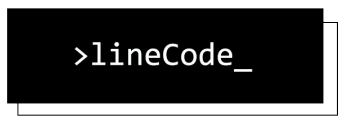
\includegraphics[scale=0.5]{../../commons/res/lclong.png} \\
			Valton Tahiraj  \\
			\textit{Responsabile di progetto}
			\href{}{}}
\address{ Via Trieste, 63 \\ Padova \\ 35121 PD, Italia}

\date{23 agosto 2021}

\begin{document}

\begin{letter}{ }

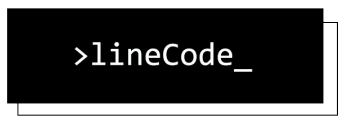
\includegraphics[scale=0.5]{../../commons/res/lclong.png}

\opening{Gentile prof. Vardanega,\\ Gentile prof. Cardin, }

Con la presente il gruppo 9, \textit{lineCode}, intende confermare la volontà di partecipare alla Revisione di Accettazione per presentarvi il prodotto completo \textbf{PORTACS (Capitolato C5)}, da Voi commissionato e proposto dall'azienda \textit{Sanmarco Informatica}. Come specificato nel Piano di Progetto v4.0.0, il costo finale del prodotto è di 13124,00\euro. \\

Vi forniamo il link di una repository pubblica da cui è possibile scaricare e visualizzare online i documenti richiesti. In particolare:

\begin{itemize}
	\item \textit{Glossario v4.0.0};
	\item \textit{Manuale Manutentore v1.0.0};
	\item \textit{Manuale Utente v1.0.0};
	\item \textit{Norme di Progetto v4.0.0};
	\item \textit{Piano di Progetto v4.0.0};
	\item \textit{Piano di Qualifica v4.0.0};
	\item \textit{Specifica dei test v1.0.0};	
	\item \textit{verbali interni ed esterni}.
\end{itemize}
Inoltre, potrete trovare il codice sorgente del prodotto finito nel Repository GitHub indicato sotto.

\newpage

Vengono anche riportati i nominativi e numeri di matricola dei membri del gruppo. Nello specifico:

\begin{center}
   \centering
   \begin{tabular}{ll}
     \textbf{Nominativo}        & \textbf{Matricola} \\
     Matteo Alba                     &  1075682 \\
	 Giacomo Bulbarelli              &  1144046 \\
	 Alessandro Chimetto             &  1142192 \\
	 Alessandro Dindinelli           &  1170457 \\
	 Lucia Fenu                      &  1125521 \\
     Paolo Scanferlato               &  1170709 \\
     Valton Tahiraj                  &  1193389 \\
   \end{tabular}
 \end{center}



Il link per scaricare e visualizzare i documenti è il seguente:

\begin{center}
\href{https://drive.google.com/drive/folders/193yY7AatYiKF6b8MC9qfJuRvbln97p5a}{Cartella condivisa su Google Drive}
\end{center}

Questo invece il link del codice sorgente del prodotto:

\begin{center}
	\href{https://github.com/lineCode-swe/portacs}{Repository GitHub}
\end{center}


Per qualunque altro chiarimento o problema, rimaniamo a Vostra completa disposizione.

\closing{Cordiali saluti,}

\vspace{3em}

\end{letter}

\end{document}
